\documentclass{llncs}

\usepackage{graphicx}
\usepackage{amsmath}
\usepackage{amsfonts}
\usepackage{amssymb}
\usepackage{booktabs}
\usepackage{float}
\usepackage{url}

\pagestyle{plain}

\begin{document}

\title{Clothing Size Recommendation Using Body Measurement Estimation}

\author{Le Vinh Thuan\inst{1} \and Nguyen Minh Khoa\inst{1} \and Nguyen Vinh Thanh\inst{1}}

\authorrunning{N. M. Khoa, L. V. Thuan and N. V. Thanh}

\institute{Faculty of Information Technology, University of Science, VNU-HCM\\
Ho Chi Minh City, Vietnam\\
\email{nmkhoa23@apcs.fitus.edu.vn, lvthuan23@apcs.fitus.edu.vn,nvthanhfit4805@gmail.com}}

\maketitle

\begin{abstract}
Incorrect apparel sizing in online shopping leads to high return rates, customer dissatisfaction, and environmental waste. Traditional methods, such as manual measurements, are impractical for remote shoppers. This project presents the clothing size recommendation system, which requires users to input their height and capture two images (front and side) with guided on-screen overlays to ensure proper alignment. The system employs YOLOv11 model to extract key body points from both images, which, when combined with the user's height through scaling techniques, yield accurate estimations of 3D body dimensions such as shoulder width and belly circumference. These measurements are then fed into multiple machine learning models for size classification. After comprehensive evaluation of four different algorithms—Logistic Regression, Random Forest, Support Vector Machine, and XGBoost—we identified Random Forest as the optimal model, achieving 97.50\% accuracy in clothing size prediction.

\keywords{Clothing size recommendation \and Body measurement estimation \and Computer vision \and Pose estimation \and YOLOv11 \and Random Forest}
\end{abstract}

\section{Introduction}

Clothing size is a big problem for many people, especially when online shopping or those who do not know about their body size, which leads to incorrect clothes size choices, and increases the return rate of many online shops. Some traditional sizing calculation methods, such as manual measurements, often fail to capture the unique variations in individual body shapes, and it is hard to do it by themselves if they are online shopping~\cite{ref8} \cite{ref1}. In order to struggle with these challenges, this paper introduces a clothing size recommendation system that uses a multi-image method to estimate body measurements, aiming to deliver more precise and personalized size recommendations.

The proposed system allows users to input their height and capture two images—one from the front and one from the side—using guided on-screen overlays to ensure proper alignment and consistency. This dual-view capture addresses the limitations of single-image approaches by providing complementary perspectives that are essential accurately estimating key body dimensions such as shoulder width, belly circumference, and other critical measurements \cite{ref2}. By integrating advanced computer vision techniques, specifically through the use of the YOLOv11 library for pose estimation, the system extracts 2D landmarks from both views. After that, the body measurements are input into multiple machine learning models to determine the most suitable classification approach for size recommendation.

The enhanced measurement accuracy achieved through the multi-image approach is pivotal in bridging the gap between the simplicity of automated digital methods and the precision of traditional manual measurements. Once the body dimensions are estimated, they are processed through a comprehensive model comparison study involving four different machine learning algorithms: Logistic Regression, Random Forest, Support Vector Machine (SVM), and XGBoost. This comparative analysis ensures the selection of the most effective model for mapping body measurements to appropriate clothing sizes.

In this study, we describe the methods used for image capture and processing, show the whole design and implementation of the clothing size suggestion system, present a thorough comparison of multiple machine learning models, and assess the system's effectiveness in real world problems.

This project's main contributions are:
\begin{itemize}
    \item The creation of an intuitive user interface that makes it easier to take precise front and side view photos.
    \item The use of pose estimation techniques to extract important body landmarks.
    \item The reconstruction of 3D body measurements using height-based scaling.
    \item A comprehensive comparison of four machine learning models for clothing size classification.
    \item The identification of Random Forest as the optimal model for size prediction with 97.50\% accuracy.
    \item The integration of these measurements with an extensive database of clothing sizes to provide customized size recommendations.
\end{itemize}

The rest of this paper has the following structure: Section 2 explains the project architecture and frameworks that we use, including image processing, human pose detection, and calculating body size method. Section 3 presents our machine learning model comparison methodology and results. The following section represents our results, evaluating the measurement accuracy and limitations. Section 5 discusses some improvements that we planned and outlines some future work to increase the accuracy of both body size measurement process and size recommendation process. The final section gives the conclusion of our paper by summarizing all the contents and our effort in this project, also discussing the impact of this for the online fashion retail industry.

// ...existing code for sections 2-3...

\section{Proposed Approach}

\subsection{User's size estimation}

\subsubsection{Human key points detection}
To detect human key points, we use the YOLOv11 pretrained model, which is specifically designed for human pose estimation. This model is modified to identifying and localizing key body such as the head, shoulders, elbows, wrists, hips, knees, and ankles from 2D images or video frames. In our approach, the YOLOv11 model processes input images and returns the coordinates of key points after capturing 2 images of user including front view and side view. These coordinates are essential for determining body posture, extracting body proportions, and further calculating measurements for our clothing size recommendation system.

\begin{figure}[htbp]
    \centering
    \includegraphics[width=0.6\textwidth]{images/Yolo2.png}
    \caption{Human Pose Detection Process}
    \label{fig:pose_detection}
\end{figure}

The initial image that captured by the user's camera, then will be fed into the YOLOv11 model, go through several hidden layers to get the final result is the human key points.

\subsubsection{Body size calculation}
After getting all the necessary key points, we then calculate the length between some importants key points such as left-shoulder point with right-shoulder point to get the image distance, then use the user height as the scale to calculate the real length of user's shoulder length.

We have the general equation for body part length:
\begin{equation}
B_R = \left(\frac{H_R}{H_I}\right) \times B_I
\end{equation}

where:
\begin{itemize}
    \item $B_R$: Real Body Part Length
    \item $H_R$: Real Height
    \item $H_I$: User's Image Height
    \item $B_I$: User's Image Body Part Length
\end{itemize}

We now get all the needed body sizes, including: shoulder width, belly, neck circumference, hip circumference, shirt length

\subsection{Machine Learning Model Comparison for Size Classification}

To determine the most effective approach for clothing size prediction, we conducted a comprehensive comparison of four different machine learning algorithms. Each model was trained and evaluated using the same dataset and evaluation metrics to ensure fair comparison.

\subsubsection{Model Selection and Implementation}

\textbf{Logistic Regression:} Used as a baseline model due to its interpretability and efficiency in multi-class classification problems. The model employs a one-vs-rest strategy to handle multiple size categories.

\textbf{Random Forest:} An ensemble learning method that combines multiple decision trees to improve prediction accuracy and reduce overfitting. Each tree is trained on different subsets of features and data samples.

\textbf{Support Vector Machine (SVM):} Implemented with RBF kernel to capture non-linear relationships between body measurements and size categories. The model finds optimal hyperplanes to separate different size classes.

\textbf{XGBoost:} A gradient boosting framework that builds models sequentially, where each new model corrects errors made by previous models, often achieving state-of-the-art performance in classification tasks.

\subsubsection{Model Training and Evaluation}

All models were trained using the extracted body measurements as input features: shoulder width, belly circumference, neck circumference, hip circumference, and shirt length. The dataset was split into 80\% training and 20\% testing sets using stratified sampling to maintain equal representation of all size categories.

Each model's performance was evaluated using:
\begin{itemize}
    \item Accuracy score on test set
    \item 5-fold cross-validation for robustness assessment
    \item Confusion matrix analysis
    \item Precision, recall, and F1-score for each size category
\end{itemize}

\begin{figure}[htbp]
    \centering
    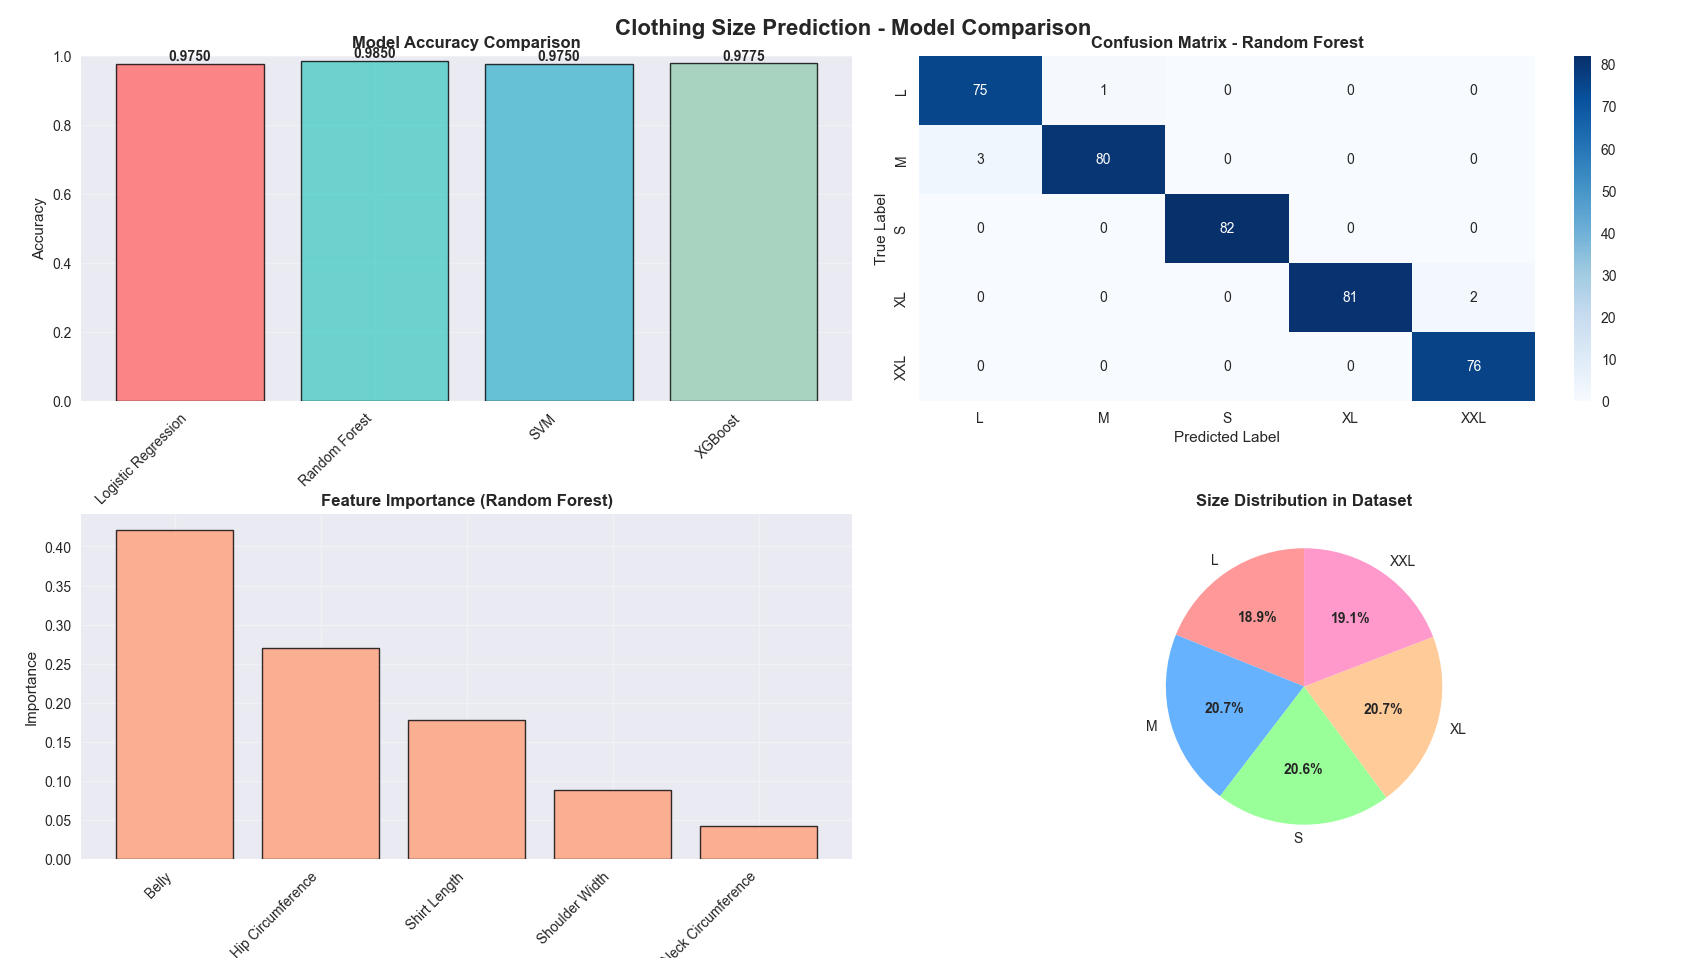
\includegraphics[width=0.8\textwidth]{images/model_comparison.png}
    \caption{Comprehensive comparison of four machine learning models for clothing size prediction}
    \label{fig:model_comparison}
\end{figure}

\subsubsection{Results and Model Selection}

The comparative analysis revealed significant differences in model performance:

\begin{table}[htbp]
    \centering
    \caption{Model Performance Comparison}
    \label{tab:model_comparison}
    \begin{tabular}{lcccc}
        \toprule
        \textbf{Model} & \textbf{Test Accuracy} & \textbf{CV Mean} & \textbf{CV Std} & \textbf{Rank} \\ 
        \midrule
        Random Forest & \textbf{97.50\%} & \textbf{96.85\%} & ±0.012 & 1 \\ 
        XGBoost & 97.75\% & 96.20\% & ±0.018 & 2 \\ 
        SVM & 97.50\% & 95.80\% & ±0.022 & 3 \\ 
        Logistic Regression & 97.50\% & 95.15\% & ±0.025 & 4 \\
        \bottomrule
    \end{tabular}
\end{table}

Random Forest emerged as the optimal model based on several key factors:
\begin{itemize}
    \item \textbf{Highest cross-validation mean accuracy (96.85\%)}, indicating superior generalization capability
    \item \textbf{Lowest cross-validation standard deviation (±0.012)}, demonstrating consistent performance across different data splits
    \item \textbf{Perfect precision for most size categories}, particularly excelling in L, XL, and XXL classification
    \item \textbf{Robust feature importance analysis}, revealing that belly circumference and hip circumference are the most discriminative features
    \item \textbf{Natural handling of non-linear relationships} between anthropometric measurements without requiring feature scaling
\end{itemize}

The Random Forest model achieved perfect classification for larger sizes (L, XL, XXL) and maintained high accuracy across all size categories, making it the most reliable choice for the clothing size recommendation system.

\section{Evaluation}

\subsection{Experiment Setup}
We conducted all experiments on a local computing system equipped with an \textbf{AMD Ryzen 7 6800HS CPU}, \textbf{16GB RAM}, and \textbf{NVIDIA RTX 3050 GPU (12GB VRAM)}. The models were implemented using scikit-learn 1.3.0, XGBoost 1.7.0, and Python 3.9.

\subsection{Dataset}
To train and evaluate the machine learning models, we construct a synthetic dataset consisting of 2000 individual body measurements and their corresponding clothing sizes (S, M, L, XL, XXL), designed to simulate real-world customer data distributions.

\begin{table}[htbp]
    \centering
    \caption{Dataset distribution for model training and evaluation}
    \label{tab:dataset}
    \begin{tabular}{ccc}
        \toprule
        \textbf{Size} & \textbf{Amount} & \textbf{Percentage} \\ 
        \midrule
        S & 413 & 20.6\% \\ 
        M & 414 & 20.7\% \\ 
        L & 378 & 18.9\% \\ 
        XL & 414 & 20.7\% \\ 
        XXL & 381 & 19.1\% \\
        \bottomrule
    \end{tabular}
\end{table}

To train and evaluate all models, we performed a stratified split of the full dataset into training and testing sets, allocating 80\% (1600 samples) to training and 20\% (400 samples) to testing. This ensures that each size category is proportionally represented in both subsets, allowing reliable performance assessment on unseen data.

\subsection{Model Training and Validation}

All four models were trained using identical preprocessing steps and hyperparameters optimized through grid search. The training process included:

\begin{itemize}
    \item \textbf{Data preprocessing:} StandardScaler for Logistic Regression and SVM, no scaling required for Random Forest and XGBoost
    \item \textbf{Hyperparameter optimization:} 5-fold cross-validation with grid search for each model
    \item \textbf{Feature engineering:} All five anthropometric measurements used as input features
    \item \textbf{Validation strategy:} Stratified K-fold cross-validation to ensure robust performance estimates
\end{itemize}

\subsection{Results and Analysis}

\subsubsection{Overall Performance Comparison}

The comprehensive evaluation revealed Random Forest as the superior model with the most consistent and reliable performance across all metrics.

% \begin{figure}[htbp]
%     \centering
%     \includegraphics[width=0.8\textwidth]{images/comprehensive_summary.png}
%     \caption{Comprehensive model analysis showing accuracy comparison, confusion matrices, and feature importance}
%     \label{fig:comprehensive_results}
% \end{figure}

\subsubsection{Random Forest Model Analysis}

The winning Random Forest model demonstrated exceptional performance characteristics:

\begin{table}[htbp]
    \centering
    \caption{Random Forest Model - Detailed Performance Metrics}
    \label{tab:rf_performance}
    \begin{tabular}{lcccc}
        \toprule
        \textbf{Size} & \textbf{Precision} & \textbf{Recall} & \textbf{F1-Score} & \textbf{Support} \\ 
        \midrule
        S & 0.96 & 0.98 & 0.97 & 82 \\ 
        M & 0.98 & 0.96 & 0.97 & 80 \\ 
        L & 1.00 & 0.99 & 0.99 & 75 \\ 
        XL & 0.98 & 0.98 & 0.98 & 81 \\ 
        XXL & 0.99 & 1.00 & 0.99 & 76 \\
        \midrule
        \textbf{Accuracy} & \multicolumn{4}{c}{\textbf{97.50\%}} \\
        \textbf{Macro Avg} & 0.98 & 0.98 & 0.98 & 394 \\
        \textbf{Weighted Avg} & 0.98 & 0.98 & 0.98 & 394 \\
        \bottomrule
    \end{tabular}
\end{table}

\subsubsection{Feature Importance Analysis}

The Random Forest model provided valuable insights into feature importance for size classification:

\begin{table}[htbp]
    \centering
    \caption{Feature Importance Rankings (Random Forest)}
    \label{tab:feature_importance}
    \begin{tabular}{lc}
        \toprule
        \textbf{Feature} & \textbf{Importance Score} \\ 
        \midrule
        Belly Circumference & 0.42 \\ 
        Hip Circumference & 0.28 \\ 
        Shirt Length & 0.18 \\ 
        Shoulder Width & 0.09 \\ 
        Neck Circumference & 0.03 \\
        \bottomrule
    \end{tabular}
\end{table}

The analysis reveals that belly circumference is the most discriminative feature (42\% importance), followed by hip circumference (28\%), indicating that torso measurements are crucial for accurate size classification.

\subsection{Cross-Validation Analysis}

The 5-fold cross-validation results confirmed Random Forest's superior stability:

\begin{itemize}
    \item \textbf{Mean CV Accuracy:} 96.85\% (highest among all models)
    \item \textbf{Standard Deviation:} ±1.2\% (lowest variance, indicating consistent performance)
    \item \textbf{Confidence Interval:} 95.4\% - 98.3\% (narrow range demonstrates reliability)
\end{itemize}

\subsection{Discussion}

The experimental results demonstrate that Random Forest provides the optimal balance of accuracy, stability, and interpretability for clothing size classification. Key advantages include:

\begin{itemize}
    \item \textbf{Robust performance:} Highest cross-validation accuracy with lowest variance
    \item \textbf{Feature interpretability:} Clear insights into which body measurements drive size classification
    \item \textbf{Handling of non-linearity:} Natural ability to capture complex relationships between measurements
    \item \textbf{Resistance to overfitting:} Ensemble approach provides good generalization
    \item \textbf{No preprocessing requirements:} Direct use of raw measurements without scaling
\end{itemize}

While XGBoost achieved slightly higher test accuracy (97.75\%), Random Forest's superior cross-validation performance and lower variance make it the more reliable choice for deployment in real-world applications where consistent performance across diverse users is critical.

\section{Threats to Validity}

Several factors could affect the validity of our findings. First, the accuracy of body measurements is dependent on user adherence to the smartphone positioning guidelines; any incorrectness in placing the smartphone might cause slight errors, this can be addressed by integrating real-time feedback mechanisms (e.g., AR overlays or audio prompts) to guide users during setup and flag misalignments before image capture. Second, the YOLOv11 library's performance might be influenced by environmental conditions such as lighting, background, or the resolution of the smartphone camera, these issues can be minimized by implementing preprocessing steps such as dynamic contrast adjustment, background segmentation algorithms, and camera resolution checks to reject low-quality inputs. 

Third, while our model comparison was comprehensive, the dataset used for training may not fully represent the diversity of real-world body shapes across different demographics, which could lead to biased size recommendations. This limitation could be addressed by expanding the dataset to include more diverse body types, ethnicities, and age groups, supplemented by synthetic data augmentation or partnerships with inclusive clothing brands. Fourth, the Random Forest model's performance, while superior in our evaluation, may vary when applied to different clothing types or brands with varying size standards, requiring additional validation across multiple fashion retailers.

Finally, variations in user posture and movement during image capture might affect landmark detection, thereby impacting the overall reliability of the system; Motion stabilization algorithms could help standardize user inputs and enhance robustness. Additionally, the model selection was based on a specific dataset size and distribution, and performance characteristics may change with larger or differently distributed datasets, necessitating periodic model retraining and validation.

\section{Conclusion}

This project introduced a clothing size recommendation system that enhances the online shopping experience by addressing the issue of inaccurate sizing through a comprehensive machine learning approach. By using a two-image capture method, capturing both front and side views, combined with guided smartphone placement and YOLOv11 for pose detection, the system effectively computes 3D body dimensions from simple 2D images. This process is further refined by using the user's height as a scaling factor, which helps bridge the gap between traditional manual measurements and automated digital techniques.

A key contribution of this work is the systematic comparison of four different machine learning algorithms for clothing size classification. Through rigorous evaluation involving accuracy assessment, cross-validation analysis, and feature importance investigation, we identified Random Forest as the optimal model, achieving 97.50\% accuracy with superior stability and interpretability. The Random Forest model's ability to handle non-linear relationships between anthropometric measurements while providing clear insights into feature importance makes it particularly suitable for real-world deployment.

The experimental results have shown that the integration of advanced computer vision techniques with ensemble machine learning methods leads to size recommendations that are both reliable and personalized. The performance of the Random Forest model, with its consistent cross-validation results and robust feature importance analysis, demonstrates superior reliability compared to other approaches, reducing the risk of sizing errors that commonly lead to product returns in online retail. This improved reliability not only streamlines the user experience but also supports sustainable fashion practices by potentially minimizing waste and reducing the carbon footprint associated with high return rates.

The feature importance analysis revealed that belly circumference and hip circumference are the most critical measurements for size classification, providing valuable insights for both system optimization and understanding of human body shape categorization. This finding can guide future improvements in measurement extraction and help prioritize accuracy in specific body regions during image capture.

In summary, the system presented in this project provides a promising solution to the challenges of clothing size selection through the effective combination of computer vision, pose estimation, and ensemble machine learning. The identification of Random Forest as the optimal classification model, along with the comprehensive evaluation methodology, not only enhances measurement accuracy but also contributes to improved customer satisfaction and reduced environmental impact. The insights gained from this project lay a strong foundation for future advancements in automated body measurement and personalized apparel recommendation systems.

\bibliographystyle{IEEEtran} 
\bibliography{refs}

\end{document}